%!TEX root = ../main.tex

\documentclass[../main.tex]{subfiles}
\begin{document}

\chapter{Multi-agent Coverage}
\label{chapter:multi_agent_coverage}

In this chapter, the multi-agent coverage problem is introduced. The problem statement is formalized in Section~\ref{section:multi_agent_problem_statement}. One of the important aspects of the algorithm is a decomposition metric used during the search algorithm. The design and analysis of this metric is in Section~\ref{section:multi_decomposition_metric}. The algorithm is proposed in Section~\ref{section:multi_algorithm}. Section~\ref{section:multi_comp_analysis} presents the computational complexity analysis of the algorithm. Lastly, Section~\ref{section:multi_simulations} presents simulations and a discussion of the results.


\section{Problem Statement}
\label{section:multi_agent_problem_statement}

%First, the general multi-agent coverage problem statement is developed. Observe that a team of robots that is tasked with coverage may contain robots with different dynamics and coverage footprints. As a result, for every robot $i$ on the team, there is a corresponding free configuration space $Q_{i,\text{free}}$, a set of feasible paths $P_i$, and a coverage map $\mathcal{M}_i(q)$. \margin{given that it is located at the point $q$?} The coverable space for each robot could\margin{don't use ``could''} then be stated as:

A multi-agent coverage task is defined over a workspace $W$ and a team of $N$ robots. The workspace $W$ represents the area to be covered. The robots on the team are tasked with coverage. Each robot on a team has the same dynamics and hence, the same free configuration space $Q_{i,\text{free}}$. Each robot also has a coverage map $\mathcal{M}_i(q)$, which maps a configuration $q$ of robot $i$ to a set of points directly under the robot's coverage footprint. The objective of the problem is to compute a path for each robot such that the entire coverable space $\mathbb{C}$ is covered and the maximum path cost amongst all robot is minimized. This objective is motivated by the following.

Complicated tasks can be solved in a distributed manner with a team of robots. This is where the overall task is divided into $N$ subtasks and assigned to $N$ robots in the team. With this setup, it is often undesirable when one robot finishes its assigned subtask much later than other robots. This leads to excessive idle times for the rest of the team and unnecessarily long execution time for the overall task. This issue can be addressed if the subtask with the longest execution time is redistributed amongst other members of the team such that the duration of the overall task is reduced. In other words, amongst a collection of $N$ subtasks, one would like to modify subtasks such that the longest duration is minimized. As an example, such cost organization was used in~\cite{carlsson2009solving} for multi-depot vehicle routing problem.

Formally, this problem is stated in Problem~\ref{problem:multi_cpp}.
\begin{problem}[Multi-agent Coverage Path Planning]
\label{problem:multi_cpp}
	Given a workspace $W$ and a team of $N$ homogeneous robots with the same coverage map, compute $\{p_1,p_2,\ldots,p_n\}$ with the following conditions:
	\begin{equation}
	\begin{aligned}
		& p_i\in P_{i},\ i=1,\dots,N,\\
		& \bigcup_{i=1,\dots,N}(\bigcup_{q\in p_i}\mathcal{M}_i(q))=\mathbb{C},\\
		& \max_{i=1,\ldots,N}\{\mathcal{E}_i(p_i)\}\text{ is minimized.}
	\end{aligned}
	\end{equation}
\end{problem}

\begin{remark}[Heterogeneous Team]
	Notice that Problem~\ref{problem:multi_cpp} is defined for a team of homogeneous robots.
	A heterogeneous team consists of robots with different dynamics, which leads to coverage spaces that vary from robot to robot. Coverage space is defined as
	\begin{equation}
		\mathcal{C}_i=\bigcup_{q\in Q_{i,\text{free}}}\mathcal{M}_i(q).
	\end{equation}
	If $\mathcal{C}_i\neq\mathcal{C}_j$ then there exists some areas in the workspace that are coverable by only one of the robots. From the coverage planner's perspective, these areas need to be identified since their coverability is conditional on the dynamics of robots. This problem is beyond the scope of this thesis; hence, the team is assumed to consist of homogeneous robots only.

	\RE
\end{remark}

\begin{remark}[Path Costs]
	The path cost $\mathcal{E}(p_i)$ is the same cost described in Section~\ref{section:single_problem_statement}:
	\begin{equation}
		\mathcal{E}(p_i)=c_1\ell(p_i)+c_2a(p_i).
	\end{equation}
	Notably, this cost consists of two components: linear and angular. 

\RE
\end{remark}

%Amongst $n$ robots in the team, these sets, $\mathcal{C}_1, \mathcal{C}_2,\ldots,\mathcal{C}_n$, may not necessarily be the same. Because of this, there are some regions in the workspace that may be accessible only by certain robots. This complicates the path planning process as the ability of a robot to cover a certain section of the workspace is conditional on the robot's dynamics. In this work, we make a simplifying assumption that if a point on the workspace is coverable by robot $i$, it is coverable by all other robots on the team. In other words, we assume that all robots have the same coverable space. That is:\todo[inline]{If we are going straight to this assumption, then the problem should just be defined for homogeneous robots.  You can use a remark to discuss the case of heterogeneity.}
%\begin{equation}
%	\mathcal{C}_1=\mathcal{C}_2=\ldots=\mathcal{C}_n=\mathbb{C}.
%\end{equation}

%The general problem is now introduced in Problem~\ref{problem:multi_cpp}.



Similar to steps taken in Chapter~\ref{section:single_problem_statement}, the Problem~\ref{problem:multi_cpp} is modified by reducing the search space for paths to a set of segmented feasible paths. The problem statement for this problem is shown in Problem~\ref{problem:multi_cpp_with_lines}.
\begin{problem}[Multi-agent Coverage Path Planning with Straight Line Segments]
\label{problem:multi_cpp_with_lines}
	Given a workspace $W$ and a team of $N$ homogeneous robots with the same coverage map, compute $\{p_1,p_2,\ldots,p_n\}$ with the following conditions:
	\begin{equation}
	\begin{aligned}
		& p_i\in P_{i,\text{segmented}},\ i=1,\dots,n,\\
		& \bigcup_{i=1,\dots,N}(\bigcup_{q\in p_i}\mathcal{M}_i(q))=\mathbb{C},\\
		%& \sum_{i=1.\dots,n}\mathcal{E}_i(p_i)\text{ is minimized}.
		& \max_{i=1,\ldots,N}\{\mathcal{E}_i(p_i)\}\text{ is minimized.}
	\end{aligned}
	\end{equation}
\end{problem}

Finally, we transform Problem~\ref{problem:multi_cpp_with_lines} into an equivalent decoupled, two step problem. First, observe that a robot $i$ traversing a path $p_i$ covers the following region $w_i$:
\begin{equation}
	w_i=\bigcup_{q\in p_i}\mathcal{M}(q).
\end{equation}
By conditions stated in Problem~\ref{problem:multi_cpp_with_lines}, a team of robots has to entirely cover the coverable space. As a result, a solution to the problem has to satisfy the following:
\begin{equation}
	\label{eq:partition_condition}
	\bigcup_{i=1,\ldots,n}w_i=\mathbb{C}
\end{equation}

Notice that equation~(\ref{eq:partition_condition}) suggests some sort of decomposition of $\mathbb{C}$. Hence, given that a few requirements are satisfied, it is possible to arrive to a solution of Problem~\ref{problem:multi_cpp_with_lines} if $w_i,i=1,\ldots,n$ are computed first followed by the computation of paths for each individual cell. The requirement for this to be true is that the computation of the decomposition has to take into account the capabilities of the robots. With our approach, we accomplish this by designing a metric $\chi$ in Section~\ref{section:multi_decomposition_metric}, which assigns an approximation cost of a path for a given polygon. Our approach consists of two decoupled subproblems: a decomposition problem and a single agent path planning problem. The first subproblem is stated in Problem~\ref{problem:workspace_allocation}.

\begin{problem}[Workspace Allocation]
\label{problem:workspace_allocation}
	Given a workspace $W$ and $N$ robots with same dynamics, compute a decomposition of $\mathbb{C}$ into $\{w_1,w_2,\dots,w_N\}$ such that
	\begin{equation}
	\begin{aligned}
		& \bigcup_{i=1,\dots,N}w_i=\mathbb{C},\\
		& \max_{i=1,\ldots,N}\{\chi_i(w_i,q^0_i)\}\text{ is minimized.}
		%& \sum_{i=1,\dots,n}\chi(w_i,q_i)\text{ is minimized}.
	\end{aligned}
	\end{equation}
\end{problem}

We note that the second subproblem is the problem solved in Chapter~\ref{chapter:single_agent_coverage} and will not be covered in this section. The rest of this chapter focuses on the decomposition problem.



%Suppose a decomposition of $\mathbb{C}$ is given with a guarantee that $\max_{i=1,\ldots,n}\{\mathcal{E}_i(p_i)\}$ would be minimized provided that all $p_i$ have the lowest possible cost. The decomposition is a set of cells $\{w_i\}$ where $\cup_{i=1}^nw_i=\mathbb{C}$. Provided with this set, one has to compute a lowest cost path $p_i$ for each $w_i$ in the decomposition for a solution to Problem~\ref{problem:multi_cpp_with_lines}.

% As such, the following problem and Problem~\ref{problem:multi_cpp_with_lines} are equivalent.
%\begin{problem}[]
%\label{problem:multi_cpp_with_lines_ii}
%	Given a workspace $W$, $n$ robots with dynamics and corresponding coverage map $\mathcal{M}_i$, compute
%	\begin{equation}
%	\begin{aligned}
%		&\{w_1,w_2,\ldots,w_n\},\\
%		&\{p_1,p_2,\ldots,p_n\}
%	\end{aligned}
%	\end{equation}
%	such that
%	\begin{equation}
%	\begin{aligned}
%		&i)& \bigcup_{i=1,\dots,n}(w_i)=\mathbb{C},\\
%		&iii) &\{p_i\in P_{\text{segmented},i}\ |\ i=1,\dots,n\},\\
%		&ii)&p_i\in w_i,\\
%		&ii)& \max_{i=1,\ldots,n}\{\mathcal{E}_i(p_i)\}\text{ is minimized,}\\
%		%& \sum_{i=1.\dots,n}\mathcal{E}_i(p_i)\text{ is minimized}.
%		&iv)&\mathcal{E}_i(p_i)\leq\mathcal{E}_i(p_j), \forall p_j\in P_{\text{segmented},i}\\
%	\end{aligned}
%	\end{equation}
%\end{problem}
%However, Problem~\ref{problem:multi_cpp_with_lines_ii} can be solved via a decoupled approach by solving two separate problems. The first problem deals with an optimal decomposition of the workspace. The second problem deals with computing the lowest cost paths for each cell in the decomposition. The first problem is shown in Problem~\ref{problem:workspace_allocation} while the second problem is just an invocation of Problem~\ref{problem:min_cost_cpp_with_lines} $n$ times. The solution to that problem is covered in Chapter~\ref{chapter:single_agent_coverage}.


\section{Decomposition Metric}
\label{section:multi_decomposition_metric}

%In this section, the design of  the metric used in the Algorithm~\ref{alg:optimization_procedure} is presented. The metric consists of three terms, which are derived and analyzed in the following subsections.

The solution to Problem~\ref{problem:multi_cpp_with_lines} is a set of cells forming a decomposition of the coverable space. The evaluation of decomposition is performed with the metric $\chi$ that assigns coverage costs to polygons. Ideally, this metric would be the real cost of a coverage path for a given cell. However, as we have shown in Chapter~\ref{chapter:single_agent_coverage}, such metric would be computationally expensive. In this chapter, we develop an approximation of such cost that is easy to compute. This metric is shown in Definition~\ref{definition:decomp_metric}. The rest of the section discusses the design of this metric. 

\begin{definition}[Decomposition Metric]
\label{definition:decomp_metric}
Given a polygonal workspace $W$ and a robot with dynamics, the partition metric $\chi:W,Q\to\mathbb{R}$ maps the workspace and the robot dynamics to an approximation of a coverage path cost in the following way:
	\begin{equation}
		%\chi(w_j,q_j^0)=c_1(\text{dist}(q^0_j,w_j)+K\text{Area}(w_j))+c_2360^o\text{Turns}(w_j).
		\chi(w_j,q_j^0)=c_1[\mathcal{F}_1(q^0_j,w_j)+\mathcal{F}_2(w_j)]+c_2\mathcal{F}_3(w_j).
	\end{equation}
Here, $w_j$ refers to a workspace assigned to robot $j$ and $q^0_j$ refers to the initial position of robot $j$.
\end{definition}

\begin{remark}[Segmented Coverage Path Structure]
The design of the metric $\chi$ is motivated by the structure of a coverage path. A coverage path $p_i$ for a robot $i$ consists of three parts. The first part is the segment of the path from the starting location of the robot to its assigned region. The second part consisting of all the straight line segments used in the segmented coverage path. The last part includes all the transition segments connecting the straight segments together as shown in Figure~\ref{fig:path_parts}. Notice that the first two parts could be used as approximations for the linear component cost of the coverage path while the thirst part could be approximating the angular component. The following subsections discuss all three components in detail. \RE
\end{remark}
%The two terms, $\ell(p_i)$ and $a(p_i)$, are the linear and angular components of the path $p_i$. The metric $\chi$ attempts to emulate this structure. To that end, the following observation about the structure of a coverage path is important. 

\begin{figure}
	\centering
	\subfile{img/chapter_5/path_parts}
	\caption{The structure of a coverage path. Orange: Segments where the robot travels to its assigned region shown in blue. Red: Path segments that are straight line segments. Yellow: path segments that are transition segments.}
	\label{fig:path_parts}
\end{figure}


\subsection{Initialization and Return Distance}
\label{subsection:init_ret_distance}

The first term in the metric $\chi$ is the term is the following: 
\begin{equation}
	\mathcal{F}_1(q^0_i,w_i)=2\min_{x\in\partial w_i}||q^0_i-x||_2.
\end{equation}

This term is designed to approximate the travel distance of a robot from its starting location to its assigned task. To demonstrate the important of this term, consider the following. A team of $N$ robots have $N$ starting locations, $q^0_1,q^0_2,\ldots,q^0_N$. Depending on the decomposition technique, the starting location of a robot may be some distance away from its assigned cell. Since this travel distance may be significant, it cannot be ignored when computing the cost of a path. For example, assume $N$ robots have equal battery charge and same dynamics. In the scenario where robot $i$ is further to its assigned cell then robot $j$, robot $i$ should be responsible for smaller cell than robot $j$. We also assume that after the completion of robot's coverage task, it is required to come back to its original starting location.

\begin{theorem}
	$\mathcal{F}_1$ is a lower bound for the actual distance from the robot's initial position to the start of the coverage path.
\end{theorem}
\begin{proof}
	Denote the combined distance from the starting location of the robot $i$, $q^0_i$, to the begging of the coverage path in $w_i$, and the distance from the end of the path to $q^0_i$ be denoted as
	\begin{equation}
		\text{dist}(q^0_i,w_i).
	\end{equation}

	Since a path $p_i$ is defined in a metric space, triangular inequality hold. Hence, the following is true:
	\begin{equation}
		\mathcal{F}_1(q^0_i,w_i)\leq2\text{dist}(q^0_i,w_i).
	\end{equation}
\end{proof}

\begin{remark}[Infeasible Paths]
The benefit of this approximation is its simplicity and ease of computation. However, it is important to note that a straight path from the starting location to the closest point on the boundary of $w_i$ may not always be feasible as it may intersect an obstacle. Therefore, a situation is possible where the distance from the starting location to the assigned region is close but in reality, requires extensive navigation through obstacles. A way to mitigate this situation is by computing the distance of a shortest feasible path to $w_i$. However, this requires utilization of visibility graphs, which is computationally expensive~\cite{planning-kinematics}.
\end{remark}

%This quantity cannot be computed prior to computing the actual coverage path because starting and end points of the coverage component are not known. The only information available is $q^0_i$ and $w_i$. However, this quantity can be approximated. This approximation is denoted by $\mathcal{F}_1(q^0_i,w_i)$ and it is a lower bound on the actual value. In this work, this is accomplished via twice the shortest Euclidean distance to $w_j$. More formally, 


\subsection{Length of Straight Line Segments}
\label{subsection:sum_straight_segments}

The second term of the metric $\chi$ is the following:
\begin{equation}
	\mathcal{F}_2(w_i)=\frac{A_{\text{actual}}-A_{\text{uncovered}}^{\max}}{r}
\end{equation}

This term is designed to approximate the length of all the straight length segments. Once the robot reaches the start of its coverage path, the coverage process begins. Recall from Chapter~\ref{chapter:single_agent_coverage} that the coverage is achieved through the type of paths called segmented paths. In Section~\ref{section:single_problem_statement}, a relation between the area of the workspace and the total length of all straight line segments is demonstrated:
\begin{equation}
	\sum_i \ell_i\approx\frac{A-nk}{r}.
\end{equation}
The area of a workspace can be used to estimate a linear component of the path cost. In this section, we show that with some modifications to the area, a lower bound estimate for the length of straight line segments can be computed cheaply.

Suppose a workspace $w_i$ is filled with non-overlapping parallel straight line segments as shown in Figure~\ref{fig:line_footprint}. Assuming that the coverage footprint has a width of $r$, then the area covered by a robot traversing a line $l_i$ is $rl_i+k$. Here, $k$ is the amount of area covered beyond the starting and stopping points of a line. These areas are associated with footprints such as a circle as demonstrated by half circles in Figure~\ref{fig:line_footprint}. The total area covered in this way is equal to
\begin{equation}
	\label{eq:covered_area}
	A_{\text{covered}} = \sum_{i=1}^n(rl_i+k).
\end{equation}

\begin{figure}
	\centering
	\subfile{img/chapter_5/area_discrepancy}
	\caption{Coverage footprints over lines.}
	\label{fig:line_footprint}
\end{figure}

\begin{remark}[$A_{\text{covered}}$ and $A_{\text{actual}}$ relation.]
Note that $A_{\text{covered}}$ is not known prior to computing the coverage path. Also note that $A_{\text{covered}}\leq A_{\text{actual}}$. This is because the area near the borders of the workspace remains uncovered as evident from Figure~\ref{fig:line_footprint}. In fact, if the uncovered area is computed then $A_{\text{covered}}$ can be calculated with the following relation:
	\begin{equation}
		A_{\text{covered}}=A_{\text{actual}}-A_{\text{uncovered}}.
	\end{equation}\RE
\end{remark}

\begin{remark}[$A_{\text{uncovered}}$ Expression]
Suppose a workspace is to be covered and is populated with some straight line segments as shown in Figure~\ref{fig:sample_area}. Note the white uncovered areas near the borders of the polygon. An expression for the are of these regions is derived here. First, observe the uncovered area generated by just one line segment as shown in Figure~\ref{fig:area_error}(a), which depicts the top half of a straight segment.

Note from Figure~\ref{fig:area_error}(b), a region of interest is a trapezoid with two parallel sides $a$ and $b$, an orthogonal segment of length $2r$, and a segment of the boundary of the polygon. The area of such a trapezoid is
\begin{equation}
	A=(a+b)r.
\end{equation}
In this case, $r$ is a constant determined by the width of the coverage footprint. However, $a$ and $b$ are determined by $r$ and $\theta$, which is the angle between that particular section of the boundary and the straight line segment as shown in Figure~\ref{fig:area_error}(b). The expressions for $a$ and $b$ are as follows:
\begin{equation}
	\begin{aligned}
		&a=r\tan{\frac{\theta}{2}},\\
		&b=r\tan\left(90^o-\frac{\theta}{2}\right).
	\end{aligned}
\end{equation}

Hence, the trapezoid area can be expressed in terms of $r$ and $\theta$ as follows:
\begin{equation}
	A=2r^2\csc{\theta}.
\end{equation}
The area of a half circle is
\begin{equation}
	\frac{\pi r^2}{2}.
\end{equation}

Therefore, the amount of area that is left uncovered one side of the straight line segment is
\begin{equation}
	A_{\text{uncovered}}=2r^2\csc\theta-\frac{\pi r^2}{2}=\frac{r^2}{2}(4\csc\theta-\pi).
\end{equation}
\RE
\end{remark}

\begin{figure}
	\centering
	\subfile{img/chapter_5/sample_area}
	\caption{Sample workspace with parallel line segments.}
	\label{fig:sample_area}
\end{figure}
\begin{figure}
	\centering
	\begin{subfigure}{0.5\linewidth}
		\centering
		\subfile{img/chapter_5/area_error}
		\caption{\label{fig:area_error_i}}
	\end{subfigure}%
	\begin{subfigure}{0.5\linewidth}
		\centering
		\subfile{img/chapter_5/area_error_i}
		\caption{\label{fig:area_error_ii}}
	\end{subfigure}
	\caption{Geometry of the uncovered area.}
	\label{fig:area_error}
\end{figure}

Note that the expression for $A_{\text{uncovered}}$ is exact and $A_{\text{uncovered}}$ is a function of $\theta$, where $\theta$ varies from one edge of a polygon to the next and the orientation of the straight line segments themselves. As such, the computation of this term requires knowing $\theta$. Next, we show an approximation to this value that gets rid of this requirement.

Suppose we compute $\theta_{\max}$ where
\begin{equation}
	\theta_{\max}=\arg\max_{\theta\in\Theta}\left(\frac{r^2}{2}(4\csc\theta-\pi)\right).
\end{equation}%
Here, $\Theta$ is a set of all possible $\theta$ that a set of lines can have with the respect to any edge of a polygon. Fortunately, by the result from Huang~\cite{Huang2001optimal}, the optimal orientation of a set of lines is orthogonal to one of the edges of a polygon. Hence, if there are $n$ edges in a polygon then $|\Theta|=n^2$.

Hence, the uncovered area can then be approximated as follows:
\begin{equation}
	A_{\text{uncovered}}^{\max}=2|S|\frac{r^2}{2}(4\csc\theta_{\max}-\pi).
\end{equation}%
Here, $|S|$ is the number of straight line segments in a workspace scaled by a factor of two to account for both ends of a line. Although $|S|$ is unknown prior to computing the coverage path, it can be approximated by the minimum altitude. This approximation is exact for convex polygons and is an over approximation for non-convex polygons. Therefore, the term is modified as follows:
\begin{equation}
	A_{\text{uncovered}}^{\max}=\ceil{\frac{\alpha_{\min}}{r}}r^2(4\csc\theta_{\max}-\pi).
\end{equation}

With an easily computable expression for $A_{\text{uncovered}}^{\max}$, the expression for the total length of straight line segments can be stated as follows:
\begin{equation}
	\mathcal{F}_2(w_i)=\frac{A_{\text{actual}}-A_{\text{uncovered}}^{\max}}{r}.
\end{equation}

\begin{theorem}[Lower Bound of Total Length of Straight Line Segments]
The term $\mathcal{F}_2(w_i)$ is a lower bound to the actual total length of straight line segments in a segmented path.
\end{theorem}
\begin{proof}
The term $A_{\text{uncovered}}^{\max}$ was computed with the value of $\theta_{\max}$ that maximizes the $A_{\text{uncovered}}$ function. Moreover, the cardinality of set $S$ is approximated by $\ceil{\frac{\alpha_{\min}}{r}}$ where $|S|\leq\ceil{\frac{\alpha_{\min}}{r}}$. Hence, the following is true:
\begin{equation}
\begin{aligned}
	&A_{\text{uncovered}}^{\max}\geq A_{\text{uncovered}},\\
	\Longrightarrow\  &\mathcal{F}_2(w_i)\leq\sum_{i=1}^Nl_i
	\end{aligned}
\end{equation}
\end{proof}


\subsection{Angular Component}
\label{subsection:angular_component}

According to the cost metric introduced in Section~\ref{section:single_problem_statement}, there are two components in the cost of a coverage path: linear and angular. The term of the approximated cost developed in Section~\ref{subsection:init_ret_distance} and Section~\ref{subsection:sum_straight_segments} both serve as approximations to the linear component. In this section, an approximation for the angular component is designed.

The angular components of a coverage path depends on the type of path itself. Some paths have a particular structure, which makes them suitable for theoretical analysis. For instance, a typical Boustrophedon path contains a set of parallel line segments connected together by transition segments. Since these parallel segments are oriented in the same direction, the transition segments must traverse at least 180$^o$ angular distance. Hence, just by knowing the number of parallel segments allows for computation of the angular distance in the whole path. As a reminder, this could be achieved by computing the altitude as demonstrated in Chapter~\ref{chapter:single_agent_coverage}. However, as shown in Chapter~\ref{chapter:single_agent_coverage}, the Boustrophedon path is not optimal for general polygons. Hence, we deviate from the altitude decomposition technique and instead focus on the shape of the polygon itself. The goal being to compute an approximation of the angular components as a function of the shape of the polygon.

For that purpose, our approach is inspired by concepts such as the medial axis of a workspace and the straight skeleton graphs as reviewed in Chapter~\ref{chapter:background}. Recall that one way to compute a straight skeleton graph is by iteratively computing \emph{contours} of a polygon. Suppose a set of contours, $\mathcal{T}$ is computed by iteratively \emph{shrinking} the boundary of the polygon by distance $r$ inwards. Then the following proposition is made.

\begin{proposition}
	Given a polygonal convex workspace $W$, suppose that the coverage angle by a Boustrophedon path is $\theta$. Then $360^o|\mathcal{T}|\leq\theta$.
\end{proposition}
\begin{proof}

The proof of this proposition starts with convex polygons. Recall the center contour introduced in Chapter~\ref{chapter:background}. The distance from any edge of the convex polygon to the center contour is $\beta$. Suppose that the minimum altitude of the convex polygon under study is $\alpha$. By construction of the center contour and the minimum altitude, the following holds, as shown in Figure~\ref{fig:skeleton_altitude}.
\begin{equation}
	\beta\leq 0.5\alpha.
\end{equation}
\simpleplot{img/chapter_5/skeleton_altitude}{Minimum altitude of a convex polygon, $\alpha$. Distance to the center contour, $\beta$.}{fig:skeleton_altitude}

However, $|\mathcal{T}|=\ceil{\frac{\beta}{r}}$ and $\theta=180^o\ceil{\frac{\alpha}{r}}$. Hence, assuming that $\frac{\alpha}{r}$ is exact then
\begin{equation}
	360^o|\mathcal{T}|\leq180^o\frac{\alpha}{r}
\end{equation}

To complete the proof, concave polygons need to be considered. Recall that any concave polygon can be decomposed into a set of convex cells. We have also demonstrated that a decomposition can be constructed that minimizes the sum of minimum altitudes over all convex cells. The sum of all minimum altitudes is related to the number of parallel line segments required for coverage. Hence, a coverage angle can also be computed. Also note that every convex cell has its own center contour. However, it was shown that $360^o\frac{\beta}{r}\leq\theta$ for convex polygons. Hence, the summation over all cells will hold as well.
\end{proof}


%When we have derived the length of the straight line segments, it turns out that it is only determined by the area of the polygon and the angle. However, no other information is captured. The amount of work required for coverage depends on the area of the workspace and its complexity. We have accounted for the area of the workspace in the previous section. In this section, we will find a relation between polygons of equal area but varying complexity as shown in Figure~\ref{fig:area_complexity}.

%\begin{figure}
%	\centering
%	\begin{subfigure}{0.5\linewidth}
%		\centering
%		\subfile{img/chapter_5/area_complexity}%
%		\caption{\label{fig:area_complexity_i}}
%	\end{subfigure}%
%	\begin{subfigure}{0.5\linewidth}
%		\centering
%		\subfile{img/chapter_5/area_complexity_b}
%		\caption{\label{fig:area_complexity_ii}}
%	\end{subfigure}
%	\caption{An example of polygons with same area but various complexity.}
%	\label{fig:area_complexity}
%\end{figure}

%The difference between the two polygons in Figure~\ref{fig:area_complexity} is the complexity. Even though they have equal areas, they have different structure.



%This quantity is computed by computing the contours of the polygon. These contours are related to the notion of straight skeletons and medial axis[CITE]. An example of the type of algorithm for computing these contours is shown in Algorithm~\ref{alg:compute_contours}.

%Suppose we run Algorithm~\ref{alg:compute_contours} and we get a set of contours, $\mathcal{E}$.
%\begin{property}[Lower Bound on Turns]
%The lower bound on the number of turns for coverage of polygon $W$ is $|\mathcal{E}|$.
%\end{property}
%To prove this property, we begin by establishing this result in convex polygons.

%In Figure~\ref{fig:concave_skeleton}, $\beta_2>\beta_1$. Hence, the number of encirclements will be determined by $\beta_2$.


\section{Area Allocation Algorithm}
\label{section:multi_algorithm}

In this section, the algorithm is presented for Problem~\ref{problem:workspace_allocation}. We begin by giving an overview of the algorithm followed by a detailed description of each procedure.

The algorithm describes a greedy optimization procedure that generates a decomposition with the minimized maximum cost. The procedure is initialized with some initial decomposition and then iteratively re-optimized through pair-wise suboptimal cuts. The process terminates when no improvements to the existing decomposition are possible. %The pair-wise optimality is ensured via a linear search over a sampled search space. The whole process is started off with an initial solution.

The main optimization procedure is shown in Algorithm~\ref{alg:optimization_procedure}. The inputs for the algorithm include a polygon described the coverable space and a set of starting positions for each robot in the coverage team. The optimization procedure is initialized with some decomposition on Line~\ref{line:multi_init_decomp}. This decomposition could be any decomposition that partitions $\mathbb{C}$ into $n$ cells. One Line~\ref{line:multi_adjacency}, the adjacency graph is computed for the decomposition. Cost are computed for all cells in the decomposition and the cell with the maximum cost is identified on Line~\ref{line:multi_cost}. On Line~\ref{line:multi_reopt_recursion}, a recursive procedure is called on the cell with the highest cost. This call returns a new decomposition where some two adjacent cells in the decomposition were re-optimized.

\begin{algorithm}
	\caption{$\text{optimization\_procedure}(\mathbb{C}, \{q^0_i\})$}
	\label{alg:optimization_procedure}
	\begin{algorithmic}[1]
		\REQUIRE Polygon $\mathbb{C}=\{Z_0,Z_1,\ldots\}$, Set of starting locations $\{q^0_i\}$
			\STATE $\mathcal{D}\gets$ some decomposition of $\mathbb{C}$ consisting of $n$ cells \label{line:multi_init_decomp}
			\REPEAT
			\STATE $\mathcal{G}\gets$ adjacency graph of $\mathcal{D}$ \label{line:multi_adjacency}
			\STATE $\chi^{\max}_i\gets$ the cost and index of highest cost vertex in $\mathcal{G}$ \label{line:multi_cost}
			\STATE $\mathcal{D}\gets\text{reopt\_recursion}(\mathcal{D},\mathcal{G}, v_i)$ \label{line:multi_reopt_recursion}
			\UNTIL{$\mathcal{D}$ stops changing}
	\end{algorithmic}
\end{algorithm}

On Line~\ref{line:multi_reopt_recursion} of Algorithm~\ref{alg:optimization_procedure}, a recursive procedure is called on the cell with the highest cost. This is because the objective is to minimize the maximum cost. However, depending on the structure of the polygon and the existing decomposition, it may not always be possible to directly re-optimize the cell with the highest cost. An example where this situation may arise is where all adjacent cells to the highest cost cell have a slightly lower cost then the maximum, which results in little room for re-optimization. These high cost adjacent cells should be attempted to be re-optimized with their respective neighbors before concluding that the re-optimization is suboptimal. This procedure is described in Algorithm~\ref{alg:reopt_recursion}.

The Algorithm~\ref{alg:reopt_recursion} takes a decomposition and a vertex representing a cell in the decomposition as inputs. For each neighboring vertex to $v_i$ that has a lower cost then $v_i$, the procedure performs the following steps. On Line~\ref{line:multi_reopt_cut}, a re-optimization cut is attempted for $v_i$ and $v_j$. If the re-optimization cut was not successful, meaning it failed to find a cut that would decrease the pair-wise maximum, then the same procedure is called on $v_j$ on Line~\ref{line:multi_recursive_call}. This procedure returns decomposition with a new cut.

\begin{algorithm}
	\caption{$\text{reopt\_recursion}(\mathcal{D}, \mathcal{G}, v_i)$}
	\label{alg:reopt_recursion}
	\begin{algorithmic}[1]
		\REQUIRE Decomposition $\mathcal{D}=\{C_0,C_1,\ldots\}$, Adjacency graph $\mathcal{G}$, Vertex $v_i$
			\FOR{$v_j\in\mathcal{N}_{v_i}$}
				\IF{$\chi(v_j)<\chi(v_i)$}
					\STATE $\mathcal{D}_{\text{new}}\gets\text{reopt\_cut}(v_i,v_j,\mathcal{D},\mathcal{G})$ \label{line:multi_reopt_cut}
					\IF{$\mathcal{D}_{\text{new}}=\mathcal{D}$}
						\STATE $\mathcal{D}_{\text{new}}\gets$reopt\_recursion($\mathcal{D},v_j$)\label{line:multi_recursive_call}
					\ENDIF
					\RETURN $\mathcal{D}_{\text{new}}$
				\ENDIF
			\ENDFOR
	\end{algorithmic}
\end{algorithm}




%\begin{algorithm}
%	\caption{$\text{optimization\_procedure}(\mathbb{C}, \{q^0_i\})$}
%	\label{alg:optimization_procedure}
%	\begin{algorithmic}[1]
%		\REQUIRE Polygon $\mathbb{C}=\{Z_0,Z_1,\ldots\}$, Set of starting locations $\{q^0_i\}$
%			\STATE $D\gets$ anchored\_area\_partition$(\mathbb{C},\{q^0_i\},\frac{1}{n})$. \label{line:area_part}
%			\STATE $\mathcal{G}\gets$ adjacency graph of $D$.
%			\STATE $M\gets\chi(q^0_i,w_i), \forall w_i\in D$.
%			\REPEAT
%				\STATE $w_a\gets w_i$ from $D$ with highest $\chi(q^0_i,w_i)$.
%				\STATE $w_b\gets$ some $w_j\in D$ adjacent to $w_a$ with lowest $\chi(q^0_j,w_j)$.
%				%\STATE $w_{\text{temp}}\gets w_a\cup b_j$
%				\STATE $w_i,w_j\gets$ equitable\_cut($w_a,w_b$).
%				\STATE Modify $M$ with new costs.%\chi(q^0_j,w_j)$ and $\chi(q^0_i,w_i)$ accordingly
%				\STATE Modify $D$ with $w_i,w_j$.
%			\UNTIL{Maximum $\chi(q^0_j,w_j)\in M$ stops decreasing}
%			\RETURN $D$
%	\end{algorithmic}
%\end{algorithm}

Algorithm~\ref{alg:reopt_cut} describes a procedure for recomputing a cut that would minimize the maximum cost. In this procedure, a search for a cut is performed over a cut space. The cut space is samples with $K$ points. The point that minimizes the maximum cost is selected and a cut is performed.
\begin{algorithm}
	\caption{$\text{reopt\_cut}(v_i, v_j, \mathcal{D},\mathcal{G})$}
	\label{alg:reopt_cut}
	\begin{algorithmic}[1]
		\REQUIRE Vertices $v_i, v_j$, Decomposition $\mathcal{D}$, Adjacency graph $\mathcal{G}$
			\STATE $c\gets$ shared edge between $v_i$ and $v_j$.
			\STATE $p_s,p_e\gets$ endpoints of $c$.
			\STATE $w_{\text{temp}}\gets \mathcal{D}(v_i)\cup\mathcal{D}(v_j)$.
			\STATE $S\gets$ cut space from $p_s$.
			\IF{$\chi(v_i)>\chi(v_j)$}
				\STATE dir$\gets$ CW \COMMENT{w.l.g assume $v_i$ is to the left of $c$}
			\ELSE
				\STATE dir$\gets$ CCW
			\ENDIF			
			\STATE $\mathcal{L}\gets$ sample $S$ with $K$ points
			\STATE $p_e^{'}\gets$ point from $\mathcal{L}$ that minimizes the maximum $\{\chi(w_a),\chi(_b)\}$
			\STATE $c^{'}\gets$ cut ($p_s,p_e^{'}$)
			\STATE $w_a,w_b\gets$cut $w_{\text{temp}}$ with $c^{'}$
			\STATE $\mathcal{D}_{\text{new}}\gets\mathcal{D}$ modified with $w_a,w_b$
			\RETURN $\mathcal{D}_{\text{new}}$
%			\FOR{each $p_i\in S$ in direction dir}
%				\STATE $w_a,w_b\gets$cut $w_{\text{temp}}$ with an edge $(p_s,p_i$)
%				\IF{dir is CW and $\chi(w_a)>\chi(w_b)$}
%					\STATE \COMMENT{Reverse inequality sign for CCW}
%					\STATE $V\gets$ sample edge($v_i,v_{i-1}$) with $K$ points
%					\STATE $v_b\gets$ point from $V$ that minimizes the maximum $\{\chi(w^{'}_a),\chi(w^{'}_b)\}$
%					\STATE $c^{'}\gets$ cut ($v_i,v_b$)
%					\STATE $w_a,w_b\gets$ cut $w_{\text{temp}}$ with $c^{'}$
%					\RETURN $w_a,w_b$
%					
%				\ENDIF
%			\ENDFOR

	\end{algorithmic}
\end{algorithm}


%\begin{algorithm}
%	%\small
%	\caption{$\text{optimization\_procedure}(\mathbb{C}, \{q^0_i\})$}
%	\label{alg:optimization_procedure}
%	\begin{algorithmic}[1]
%		\REQUIRE Polygon $\mathbb{C}=\{Z_0,Z_1,\ldots\}$, Set of starting locations $\{q^0_i\}$
%			%\STATE $V\gets n$ virtual starting locations placed randomly on the boundary of $P$ \label{line:1_start_locs}
%			\STATE $D\gets$ anchored\_area\_partition$(\mathbb{C},\{q^0_i\},\frac{1}{n})$ \label{line:area_part}
%			\STATE $\mathcal{G}\gets$ adjacency graph of $D$
%			\STATE $M\gets\chi(q^0_i,w_i), \forall w_i\in D$ 
%			%\STATE Add all cells in $D$ to the queue $Q$
%			\REPEAT
%				\STATE $w_a\gets w_i$ from $D$ with highest $\chi(q^0_i,w_i)$
%				\STATE $w_b\gets$ some $w_j\in D$ adjacent to $w_a$ with lowest $\chi(q^0_j,w_j)$
%				\STATE $w_{\text{temp}}\gets w_a\cup b_j$
%				\STATE $\Delta\chi\gets\frac{|\chi_2-\chi_1|}{\chi_2+\chi_1}$
%				\STATE $A_t\gets$ Half of area of $w_{\text{temp}}$
%				\STATE $w_i,w_j\gets$ anchored\_area\_partition($w_{\text{temp}},(q^0_i,q^0_j),(A_t+\Delta\chi,A_t-\Delta\chi)$\label{line:distr_opt_cut}
%				%\STATE $\mathbb{E}\gets$ \text{compute\_encirclements}$(p_{\operatorname{temp}})$ \label{line:compute_encirlment}
%				%\STATE $\sigma_{\ell}\gets$ compute\_encirclements($p_{\ell}$) \label{line:recalc_encirclemnts_1}
%				%\STATE $\sigma_r\gets$ compute\_encirclements($p_r$) \label{line:recalc_encirclemnts_2}
%				%\STATE $\sigma_{\ell}\gets$ recalc\_encirclements($p_{\ell},\mathbb{E}, c$) \label{line:recalc_encirclemnts_1}
%				%\STATE $\sigma_r\gets$ recalc\_encirclements($p_r, \mathbb{E}, c$) \label{line:recalc_encirclemnts_2}
%				%\STATE Cost $\gets\chi(s_i,p_{\ell},\sigma_{\ell})+\phi(s_j,p_r,\sigma_r$) 
%				%\STATE Cost $\gets\max\{\chi(s_i,p_{\ell}),\chi(s_j,p_r)\}$ 
%				%\STATE Implement $c$ that resulted in lowest cost, modify $D$.
%				\STATE Modify $\chi(q^0_j,w_j)$ and $\chi(q^0_i,w_i)$ accordingly
%				\STATE Modify $D$ with $w_i,w_j$
%			\UNTIL{Maximum $\chi(q^0_j,w_j)\forall w_j\in D$ stops decreasing}
%			\RETURN $D$
%	\end{algorithmic}
%\end{algorithm}

Throughout the algorithm, the metric $\chi$ is used extensively. The metric is analyzed in Section~\ref{section:multi_decomposition_metric}. Algorithm~\ref{alg:metric_algorithm} demonstrates the procedure for computing the metric. The values used in the computation of this metric are described in more details in Section~\ref{section:multi_decomposition_metric}. In this algorithm, values $\mathcal{F}_1,\mathcal{F}_2$, and $\mathcal{F}_3$ are computed. 

\begin{algorithm}
	\caption{$\text{compute\_}\chi(q^0, w)$}
	\label{alg:metric_algorithm}
	\begin{algorithmic}[1]
		\REQUIRE Initial position $q^0$, Polygon $w=\{Z_0,Z_1,\ldots\}$ 
		\STATE $\mathcal{F}_1\gets2\min_{x\in\partial w}||q^0-x||_2$
		\STATE $A_\text{actual}\gets$ area of $w$
		\STATE $\Theta\gets$ angles of all edges w.r.t. the $x$-axis.
		\STATE $\theta_{\max}\gets$ largest difference between any two pairs of elements of $\Theta$
		\STATE $A^{\max}_{\text{uncovered}}\gets\alpha_{\min}r(4\csc{\theta_{\max}}-\pi)$
		\STATE $\mathcal{F}_2\gets\frac{A_\text{actual}-A^{\max}_{\text{uncovered}}}{r}$
		\STATE $\mathcal{T}\gets$ compute\_contours of $w$
		\STATE $\mathcal{F}_3\gets360^o|\mathcal{T}|$
		\RETURN $c_1(\mathcal{F}_1+\mathcal{F}_2)+c_2\mathcal{F}_3$
	\end{algorithmic}
\end{algorithm}

%Another important sub-procedure is the call to anchored area partition procedure. This procedure is based on the work by Hert~\cite{hert1998polygon} and his approach to area partitioning problem. The procedure is summarized in Algorithm~\ref{alg:anchored_area_partition}. This algorithm allows for making cuts without having to discretized the coverable area. Moreover, a series of cuts are made to form $n$ cells with area specified as an input to the algorithm. For brevity, we only show the algorithm for convex polygons here. The full algorithm will be available in the Appendix.

%\begin{algorithm}
%	\caption{$\text{anchored\_area\_partition}(w, (q^0_i,q^0_j), A_1,A_2)$}
%	\label{alg:anchored_area_partition}
%	\begin{algorithmic}[1]
%		\REQUIRE Polygon $w=\{Z_0,Z_1,\ldots\}$, Tuple of starting locations $(q_i,q_j)$, tuple of required areas
%		\STATE $V(w)\gets$ list of vertices in CCW order
%		\STATE Order $q^0_i,q^0_j$ according to this order as well
%		\STATE Initialize the cut $L=(L_s,L_e)$ as an edge $(v_0,q^0_1)$
%		\WHILE{$\text{Area}(w_j)<A_2$ or $L_e!=q^0_2$}
%			\STATE Move $L_e$ CCW
%		\ENDWHILE
%		\IF{$\text{Area}(w_j)<A_2$}
%			\WHILE{$\text{Area}(w_j)<A_2$}
%				\STATE Move $L_s$ CW
%			\ENDWHILE
%		\ENDIF
%		\RETURN $w_i,w_j$
%	\end{algorithmic}
%\end{algorithm}

%In Algorithm~\ref{alg:optimization_procedure}, in Line~\ref{line:compute_encirlment}, a procedure is called to compute \emph{encirclements}. The procedure for computing them is shown in Algorithm~\ref{alg:compute_contours}.
%\begin{algorithm}
%	\small
%	\caption{$\operatorname{compute\_encirclements}$}
%	\label{alg:compute_contours}
%	\begin{algorithmic}[1]
%		\REQUIRE Polygon $P=\{Z_0,Z_1,\ldots\}$
%		\STATE $\mathcal{C}\gets\emptyset$ 
%		\REPEAT
%			\STATE $C\gets$ \textit{parallel\_offset\_inwards}$(P)$
%			\STATE $\mathcal{C}\gets C$
%		\UNTIL{No further shrinking possible}
%		\RETURN $\mathcal{C}$
%	\end{algorithmic}
%\end{algorithm}
%
%The Algorithm~\ref{alg:update_contours} shows a procedure for recalculating the number of encirclements to avoid constant re-computation of contours. This increases the efficiency of the algorithm.
%\begin{algorithm}
%	\small
%	\caption{$\operatorname{recalc\_encirclements}$}
%	\label{alg:update_contours}
%	\begin{algorithmic}[1]
%		\REQUIRE Polygon $P=\{Z_0,Z_1,\ldots\}$, Set of contours $\mathbb{E}$, cut $c$
%		\STATE $\mathcal{C}\gets\emptyset$ 
%		\REPEAT
%			\STATE $C\gets$ \textit{parallel\_offset\_inwards}$(P)$
%			\STATE $\mathcal{C}\gets C$
%		\UNTIL{Shrinking results in a point or line}
%		\RETURN $\mathcal{C}$
%	\end{algorithmic}
%\end{algorithm}


\section{Computational Complexity}
\label{section:multi_comp_analysis}

In this section, we perform a computational complexity analysis of the algorithm. Line 1 of Algorithm 7 is performed in $\mathbb{O}(n)$ by iterating over all vertices. Similarly the area of a polygon is computed in $\mathbb{O}(n)$ time. Lines 3 $\mathbb{O}(n)$ have similar execution time. Line 4 is $\mathbb{O}(n^2)$ since all pairs of edges have to be examined. On Line 7, the contours are being computed. The computation of a contours is performed by repeatedly shrinking the boundary of a polygon. Although we use the Shapely library for this, it can be theoretically performed with following steps. 

Computing contours can be done via a simple algorithm proposed by Chen~\cite{chen2005polygon}, which is done in $\mathbb{O}((n+k)\log{n})$



\section{Simulations}
\label{section:multi_simulations}

Our decomposition algorithm was implemented in Python. The algorithm was implemented with the help of computational geometry libraries including Shapely~\cite{Shapely:13} and Visilibity\cite{VisiLibity:08}. The heuristic solver GLKH~\cite{helsgaun2000effective} was used as a GTSP solver. Transition costs between segments were computed assuming a Dubins' vehicle model~\cite{dubins1957curves}.

%Our method was compared to two other approaches. In the first method we use an approximate point decomposition of the workspace from~\cite{arkin2000approximation}. Each point is assigned eight headings. These headings represent possible traversal directions for that point. Finally, the GTSP tour of minimum cost is computed as in%~\cite{le2012dubins}. In the second method, we compute the coverage path as in Section~\ref{sec:gtsp_tour}, but where the re-optimization procedure is not performed on the initial decomposition. For the initial decomposition, a Python library for greedy convex decomposition is used, based on~\cite{fernandez2008practical}. We tested all approaches on four different workspaces of similar size but various complexity. The workspaces are based on test environments used in~\cite{choi2009online}.


\begin{table}
	\centering
	\caption{Decomposition methods comparison for multiple test shapes.}
	\label{table:performance}
	\begin{tabular}{@{} l rrrr l rrrr l rrrr l@{}}
		\toprule
		&& Size & Time & Length & Area \\
		\cmidrule{3-6}
		\multirow{4}{*}{Point Decomposition} & Shape 1 & 7144 & 2h & 312.6 & 87.8\%\\
		& Shape 2 & 7288  & 2h & 306.3 & 86.9\%\\
		& Shape 3 & 7464 & 2h & 349.3 & 88.3\%\\
		& Shape 4 & 6736 & 2h & 312.2 & 85.1\%\\
		%\midrule
		%\multirow{4}{*}{Greedy Decomposition} & Shape 1 & 96 & \bf{2s} & \bf{231.0} & 91.6\%\\
		%& Shape 2 & 86 & \bf{2s} & \bf{216.8} & 84.6\%\\
		%& Shape 3 & 136 & \bf{6s} & \bf{226.9} & 79.8\%\\
		%& Shape 4 & 116 & \bf{3s} & \bf{226.5} & 88.1\%\\
		%\midrule
		%\multirow{4}{*}{Min Alt Decomposition} & Shape 1 & \bf{78} & 2s & 242.3 & \bf{95.1\%}\\
		%& Shape 2 & \bf{80} & 7s & 228.9 & \bf{91.7\%} \\
		%& Shape 3 & \bf{92} & 15s & 228.1 & \bf{89.1\%} \\
		%& Shape 4 & \bf{88} & 13s & 234.4 & \bf{93.5\%}\\
		\bottomrule

	\end{tabular}
\end{table}


%Performance figures of all three methods are shown in Table~\ref{table:performance}. We compare four characteristics of the three approaches: 1) the size of the GTSP instance, 2) the execution time from start to finish, 3) the total length of the tour, and 4) the area covered by the coverage path as percentage of the total area of the polygon. We note that in all four test shapes, our method reduced the number of turns in the final coverage path. This is shown in the reduction in GTSP size, which is equivalent to the reduction in number of straight line segments. Naturally, since our method uses greedy decomposition as a starting point, it runs more slowly then the pure greedy approach. On average, out method is about three times slower than the greedy approach. However, it is faster then the point decomposition by a factor of 100. 

%It is worth noting that the overall path lengths are slightly shorter with the greedy decomposition compared to our method. However, this factor is mostly attributed to the fact that greedy decomposition produces many regions whose area is small relative to the size of the footprint. These regions are typically very narrow, which makes it difficult to place lines inside those regions that cover most of the area. Decompositions that produce excessive number of such regions results in a significant portion of the total area of the polygon uncovered. Our method produces fewer regions and leaves less area uncovered. From Table~\ref{table:performance}, the uncovered area left by our method is on average half of the uncovered area left by the greedy approach. It is worth noting that point decomposition in some cases covers less area than the competing algorithms. However, this occurrence is primarily due to our method for generating the approximate decomposition, which does not place any coverage footprints at a distance of less than $r$ from the boundary, leading to uncovered areas near polygon boundaries.

%Figure~\ref{fig:coverage_results} shows the resultant paths for three different approaches. The line segments are orange and green segments show Dubins transition costs. Note that green segments do not necessarily indicate the path of the robot but rather show the cost associated with the transition. The red lines highlight shared edges of adjacent polygons in the decomposition. The first column of figures show the point decomposition. The second column of figures show the greedy decomposition technique. And the last column shows our re-optimization technique. 

%From Figure~\ref{fig:coverage_results} we can see that our method significantly reduces the number of polygons compared to the greedy decomposition. Inefficiencies in the GTSP tour occur due to the very large size of the GTSP instance, which poses a challenge for the heuristic GLKH solver.



\begin{figure*}
		\centering
		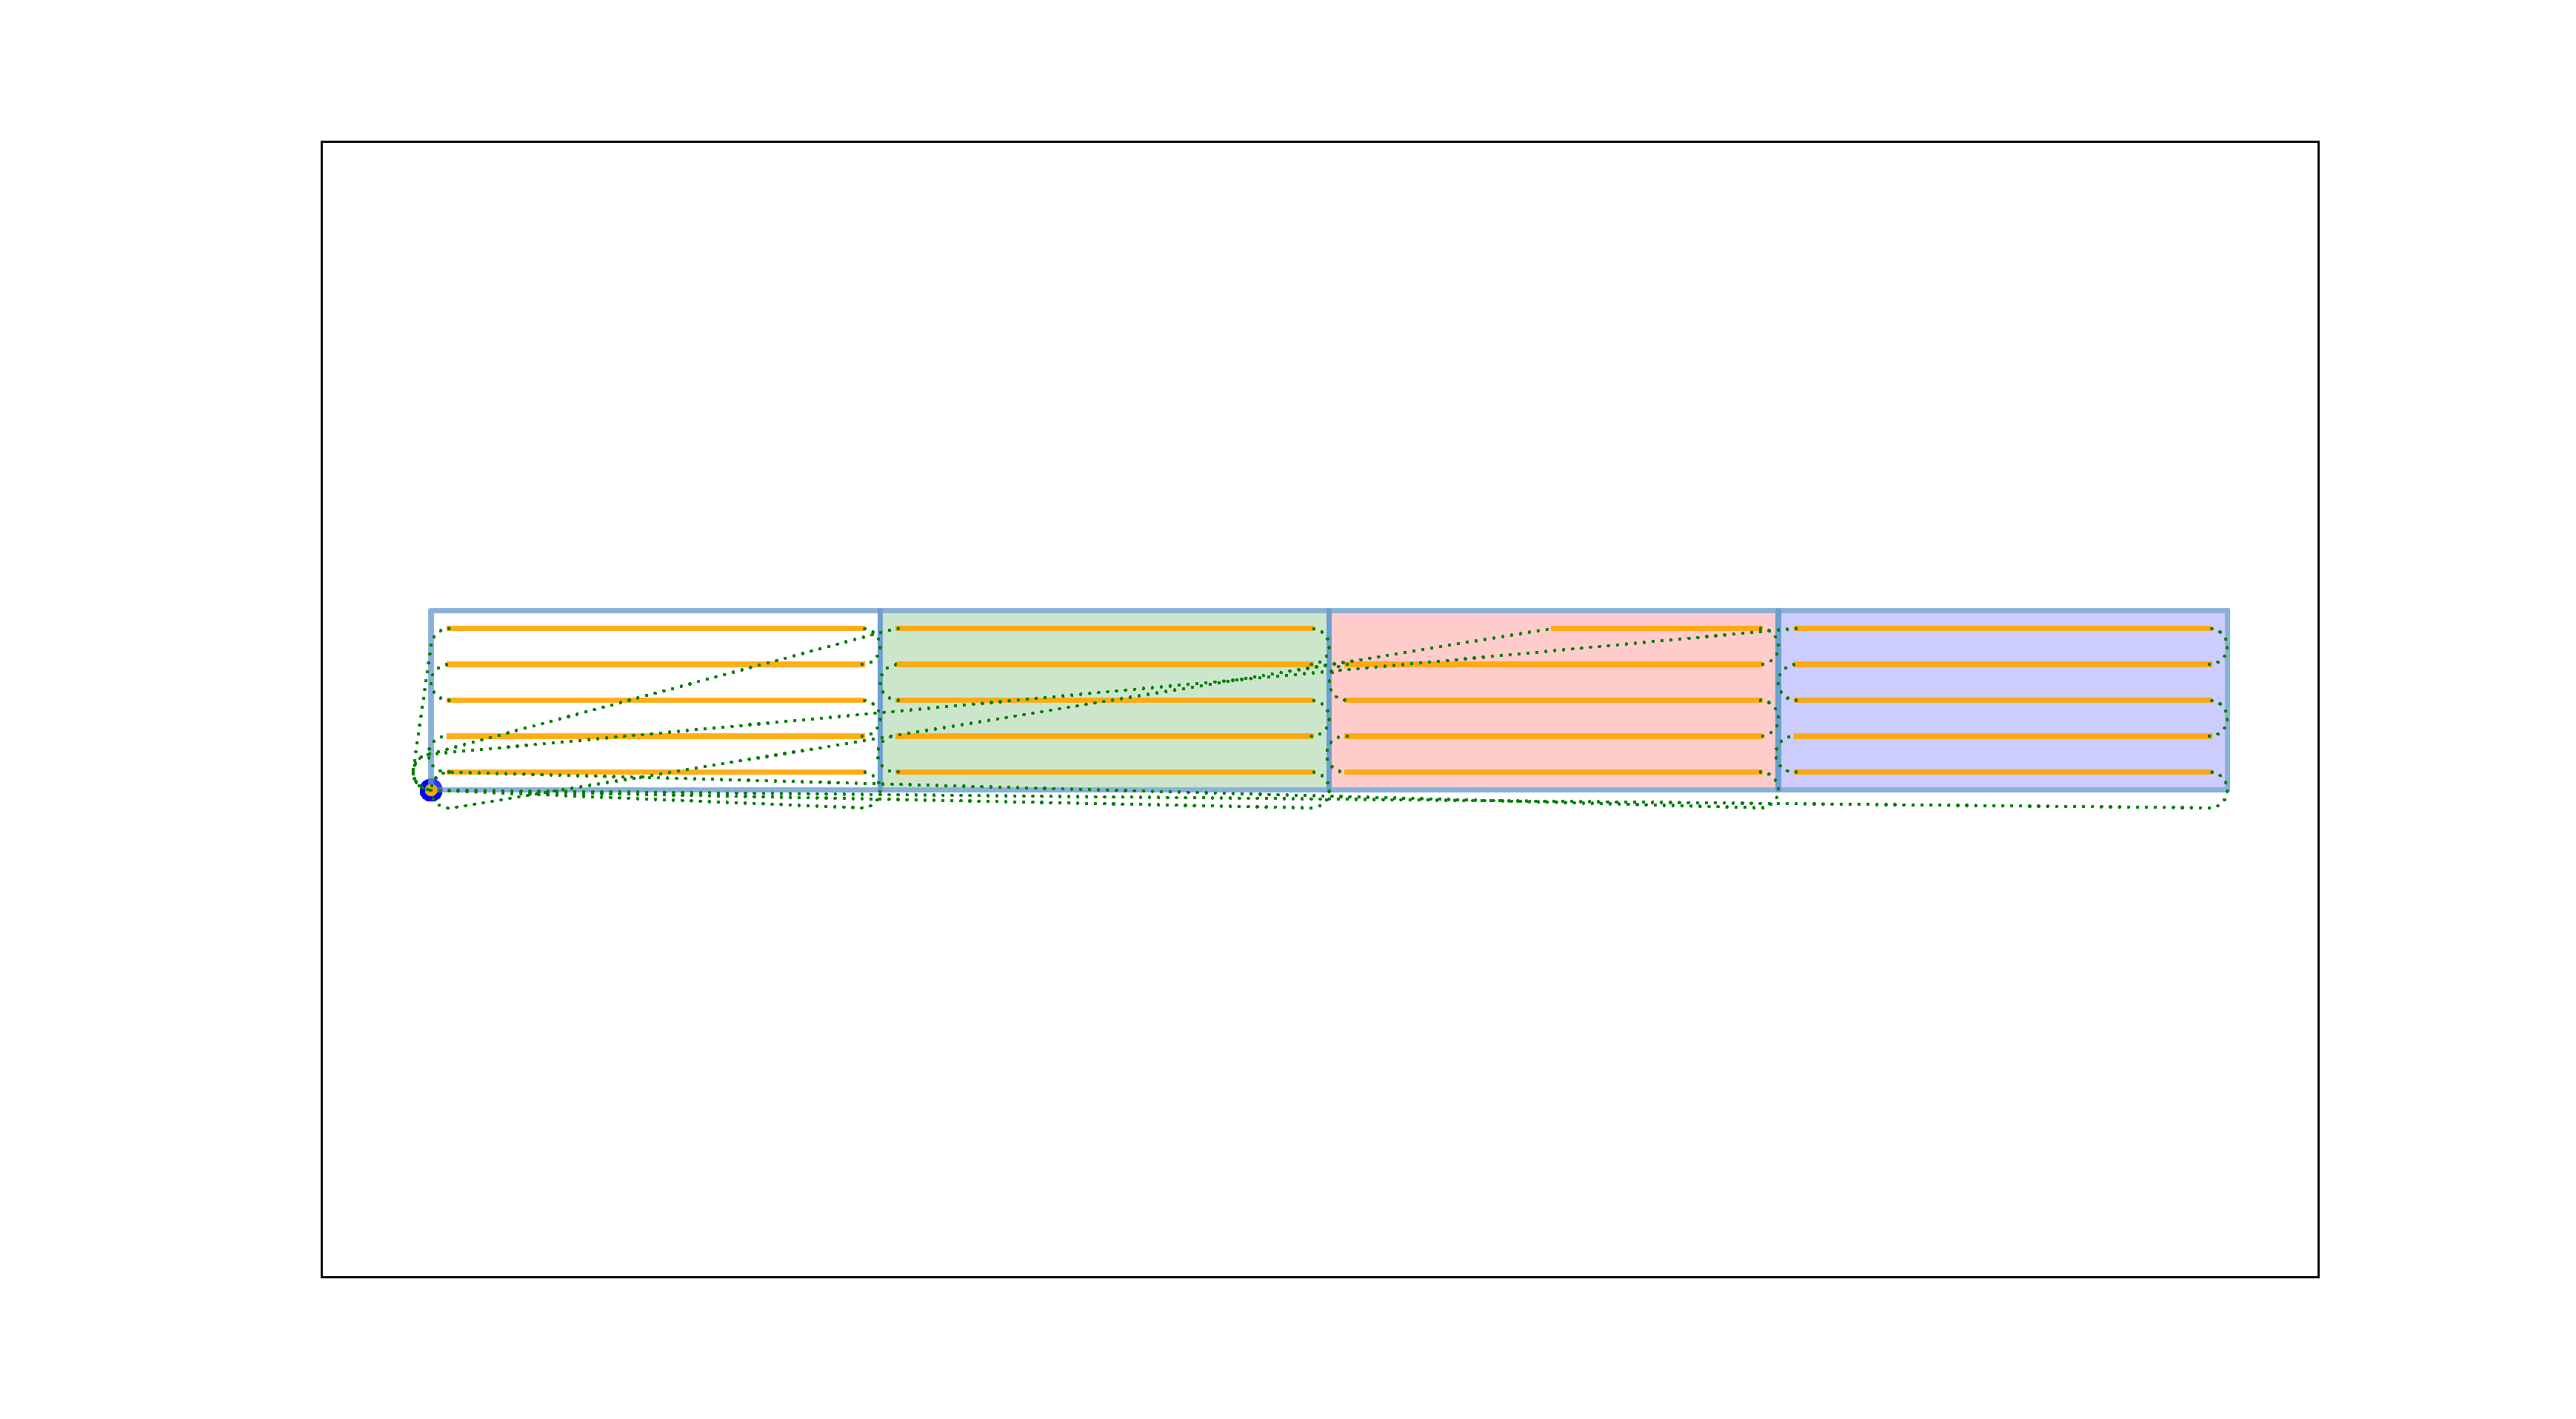
\includegraphics[width=0.45\textwidth]{img/chapter_5/ID_1_orig.pdf}% 
		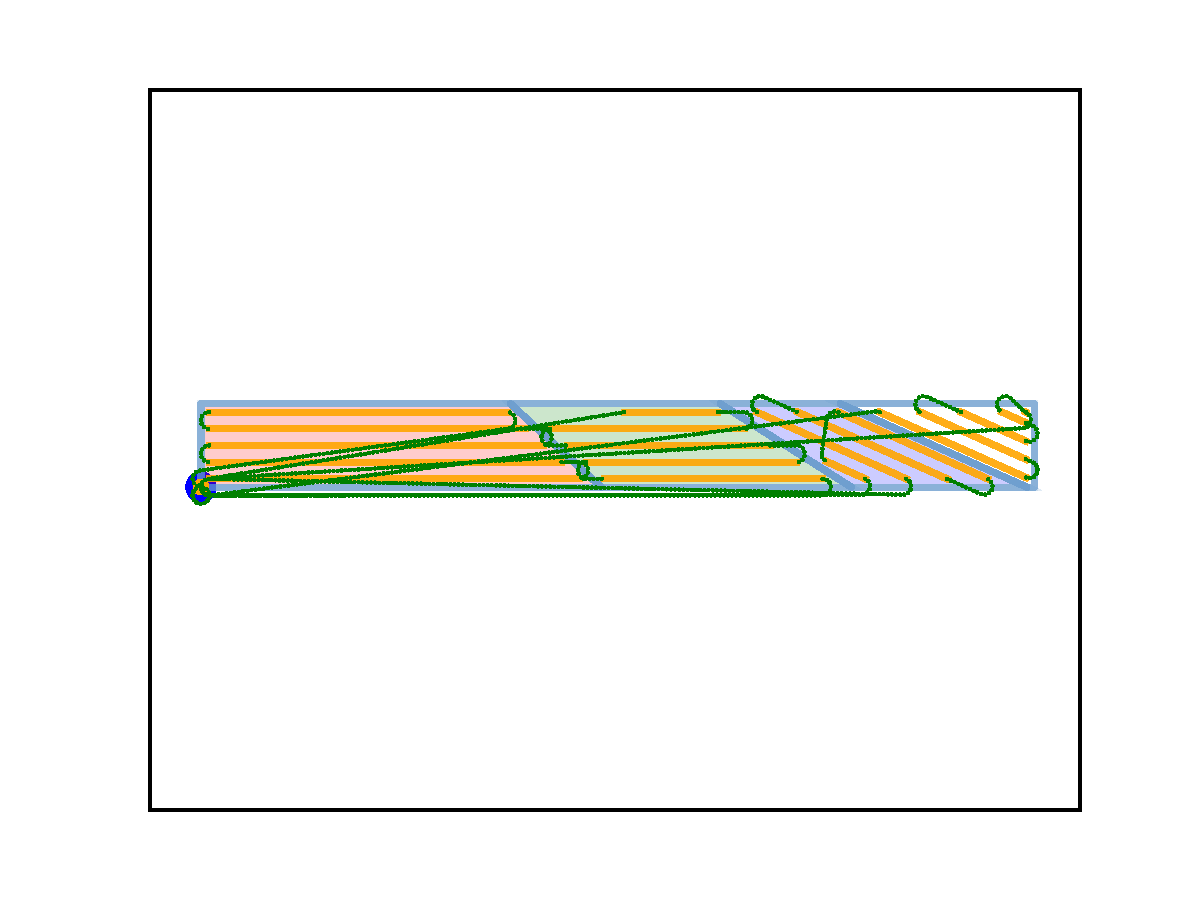
\includegraphics[width=0.45\textwidth]{img/chapter_5/ID_1_reopt.pdf}

		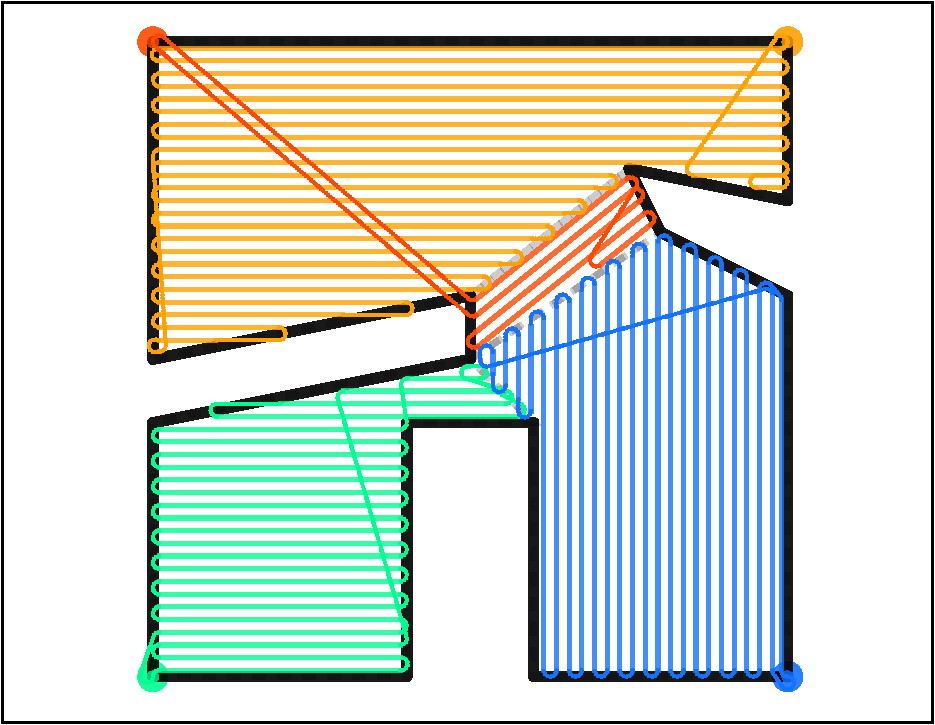
\includegraphics[width=0.45\textwidth]{img/chapter_5/ID_2_orig.pdf}% 	
		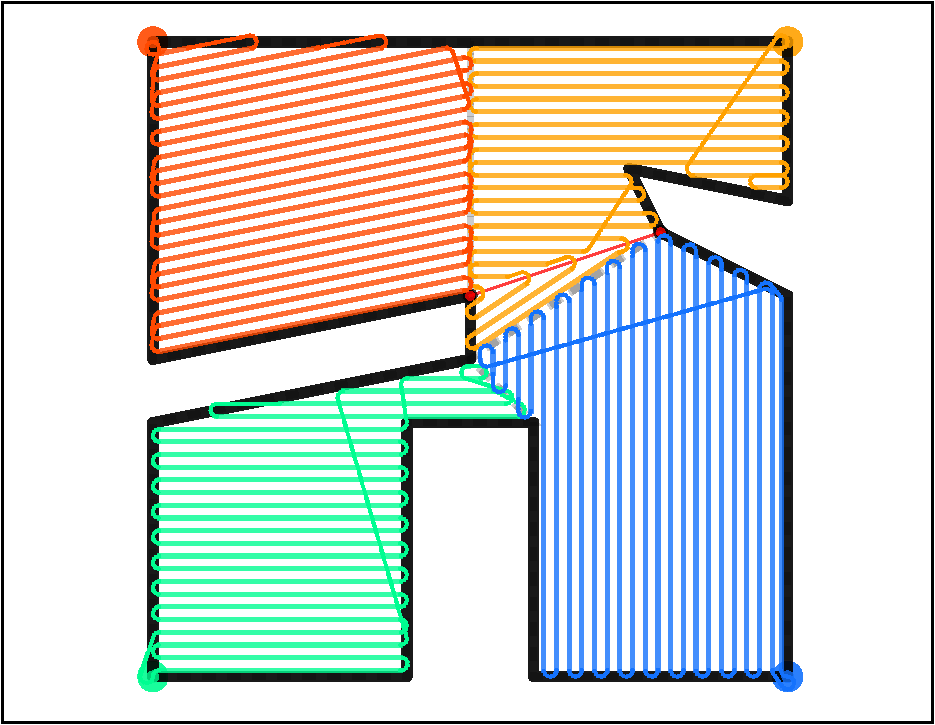
\includegraphics[width=0.45\textwidth]{img/chapter_5/ID_2_reopt.pdf}

		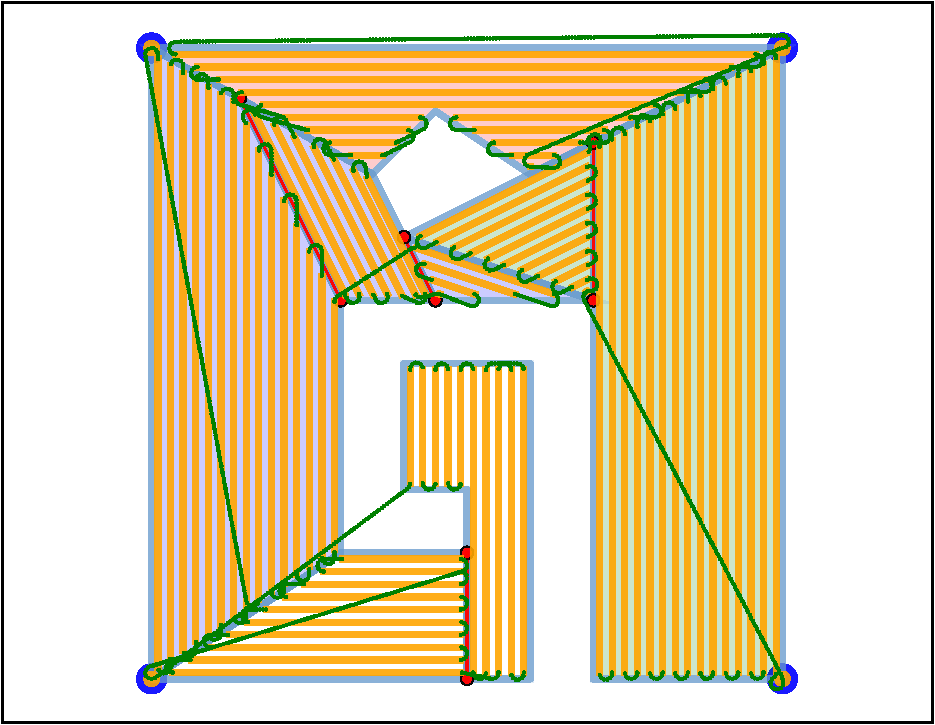
\includegraphics[width=0.45\textwidth]{img/chapter_5/ID_3_orig.pdf}%
		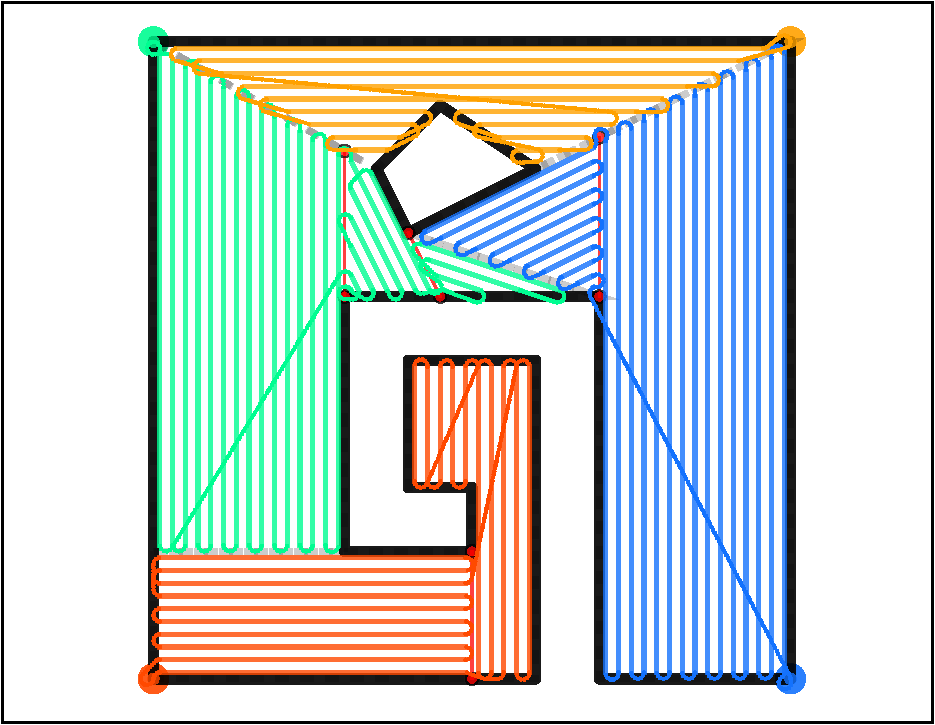
\includegraphics[width=0.45\textwidth]{img/chapter_5/ID_3_reopt.pdf}

	\caption{First column: decomposition before re-optimization. Second column: after re-optimization.}
	\label{fig:decomposition_results}
\end{figure*}


\end{document}